\subsubsection[多变量函数的极限]{Limit}
\begin{define}[Limit]
    Let $f:\,D\left(\subseteq\mathbb{R}^2\right)\to\mathbb{R}$, $M_0$ is an accumulation point of $D$. If for some $a\in\mathbb{R},\,\forall\varepsilon>0,\,\exists\delta=\delta(\varepsilon)>0$ s.t. $\forall M\in D\cap B^-\left(M_0,\delta\right),\,\left|f(M)-a\right|<\varepsilon$, then we say $f$ converges to $a$ as $M$ converges to $M_0$, simply denote it by $\lim_{M\to M_0}f(M)=a$.
\end{define}

$\forall\varepsilon>0,\,\exists\delta=\delta(\varepsilon)>0$, s.t. $\forall(x,y)\in D,\,(x,y)\neq M_0=\left(x_0,y_0\right),\,\left|x-x_0\right|<\delta,\,\left|y-y_0\right|<\delta,\,\left|f(x,y)-a\right|<\varepsilon$

$$
    \text{(}\lim_{
        \underset{\substack{\downarrow\\\lim_{y\to y_0}\lim_{x\to x_0}f(x,y)\text{ 累次极限}\\\lim_{M_0+tv}f\left(M_0+tv\right)}}{\substack{x\to x_0\\y\to y_0}}}f(x,y)\text{)}
$$

Similarly, we can define $\lim_{\substack{x\to\infty\\y\to\infty}}f(x,y),\,\lim_{\substack{x\to x_0\\y\to\infty}}f(x,y),\,\dots$

\begin{example}
    \begin{enumerate}
        \item Prove $\lim_{(x,y)\to(0,0)}\frac{x^2y^2}{x^4+y^2}=0$
              \begin{pf}
                  $\left|\frac{x^2y^2}{x^4+y^2}\right|=|y|\left|\frac{x^2y}{x^4+y^2}\right|\leq\frac{1}{2}|y|$

                  $\forall\varepsilon>0,\,\exists\delta=\varepsilon$ s.t. $\forall(x,y)\in\mathbb{R}^2\setminus\left\{(0,0)\right\},\,|x|<\delta,\,|y|<\delta$

                  $\left|\frac{x^2y^2}{x^4+y^2}\right|\leq\frac{1}{2}|y|<\varepsilon$

                  Q.E.D.
              \end{pf}
        \item Prove $\lim_{(x,y)\to(0,0)}\frac{x^3+y^3}{x^2+y^2}=0$ ($\left|\frac{x^3+y^3}{x^2+y^2}=0\right|\leq|x|+|y|$)
        \item Consider $f(x,y)=\frac{x^2y}{x^4+y^2},\,(x,y)\neq(0,0)$

              $\lim_{y\to 0}\lim_{x\to 0}\frac{x^2y}{x^4+y^2}=0\quad\lim_{x\to 0}\lim_{y\to 0}\frac{x^2y}{x^4+y^2}=0$

              $$
                  f(x,y)=f(x,kx)=\frac{x^2\cdot kx}{x^4+k^2x^2}=\frac{k}{k^2+x^2}x\to 0\text{, as }x\to 0
              $$

              \allbold{If we consider $y=kx^2,\,f(x,y)=f\left(x,kx^2\right)=\frac{x^2\cdot kx^2}{x^4+k^2x^4}=\frac{k}{1+k^2}\to\frac{k}{1+k^2}\,(x\to 0)$}

              \allbold{$\implies\lim_{(x,y)\to(0,0)}\frac{x^2y}{x^4+y^2}$ does not exist}
    \end{enumerate}
\end{example}

\begin{thm}
    Suppose $f$ is defined on $B^-\left(M_0,r\right)$, then $\lim_{M\to M_0}f(M)=a\iff$ for any continuous curve $\gamma:\,(0,\delta)\to B^-\left(M_0,r\right)$ with $\lim_{t\to 0^+}\gamma(t)=M_0$, we have $\lim_{t\to 0}f\left(\gamma(t)\right)=a$
    \begin{pf}
        ``$\implies$'' $\forall \varepsilon>0,\,\exists\delta>0$ s.t. $\forall M\in B^-\left(M_0,\delta\right),\,\left|f(M)-a\right|<\varepsilon$. Then for any $\gamma:\,(0,\delta)\to B^-\left(M_0,r\right)$ with $\gamma(t)\to M_0\,(t\to 0)$. $\exists\eta>0$ s.t. $\forall 0<t<\eta,\,\gamma(t)\in B^-(M_0,\delta)$, then $\left|f\left(\gamma(t)\right)\right|<\varepsilon$

        ``$\impliedby$'' Argue by contradiction. Suppose $\lim_{M\to M_0}f(M)\neq a$, then $\exists\varepsilon_0>0$ and $\left\{M_n\right\}\subseteq B^-\left(M_0,r\right)\text{ s.t. }M_n\to M_0\,(n\to+\infty)$, and $\left|f\left(M_n\right)-a\right|\geq\varepsilon_0$

        \allbold{Construct a $\gamma:\,(0,1)\to B^-\left(M_0,r\right),\,\gamma\left(\frac{1}{2^n}\right)$ and $\gamma(t)\to M_0\,(t\to 0)$, but $f\left(\gamma\left(\frac{1}{2^n}\right)\right)=f\left(M_n\right)\not\to a$. Contradiction.}
    \end{pf}
\end{thm}

\begin{prop}[Algebraic Rules]
    If $\lim_{M\to M_0}f(M),\,\lim_{M\to M_0}g(M)$ both exists, then $\lim_{M\to M_0}(f\pm g)(M),\,\lim_{M\to M_0}(f\cdot g)(M)$ exists and $\lim_{M\to M_0}(\frac{f}{g})(M)$ exists provided $\lim_{M\to M_0}g(M)\neq0$.
\end{prop}

\begin{prop}[Heine Principle]
    Suppose $M_0$ is an accumulation point of $D$, then $\lim_{M\to M_0}f(M)=a$ iff for any point sequence $\left\{M_n\right\}\subseteq D\setminus\left\{M_0\right\}$, such that $M_n\to M_0\,(n\to+\infty)$, we have $f\left(M_n\right)\to a\,(n\to+\infty)$
\end{prop}

$\lim_{M\to M_0}f(M)$ exists $\iff\lim_{\delta\to 0}\sup_{B^-\left(M_0,\delta\right)}\left|f(M)-f\left(M'\right)\right|=0\iff$ In particular, $\lim_{\delta\to 0}\sup_{\partial B\left(M_0,\delta\right)}\left|f(M)-f\left(M'\right)\right|=0$

\begin{example}
    $f(x,y)=\begin{cases}
            \frac{xy}{x^2+y^2} & (x,y)\neq(0,0) \\
            0                  & (x,y)=(0,0)
        \end{cases}$\quad\raisebox{-0.5\height}{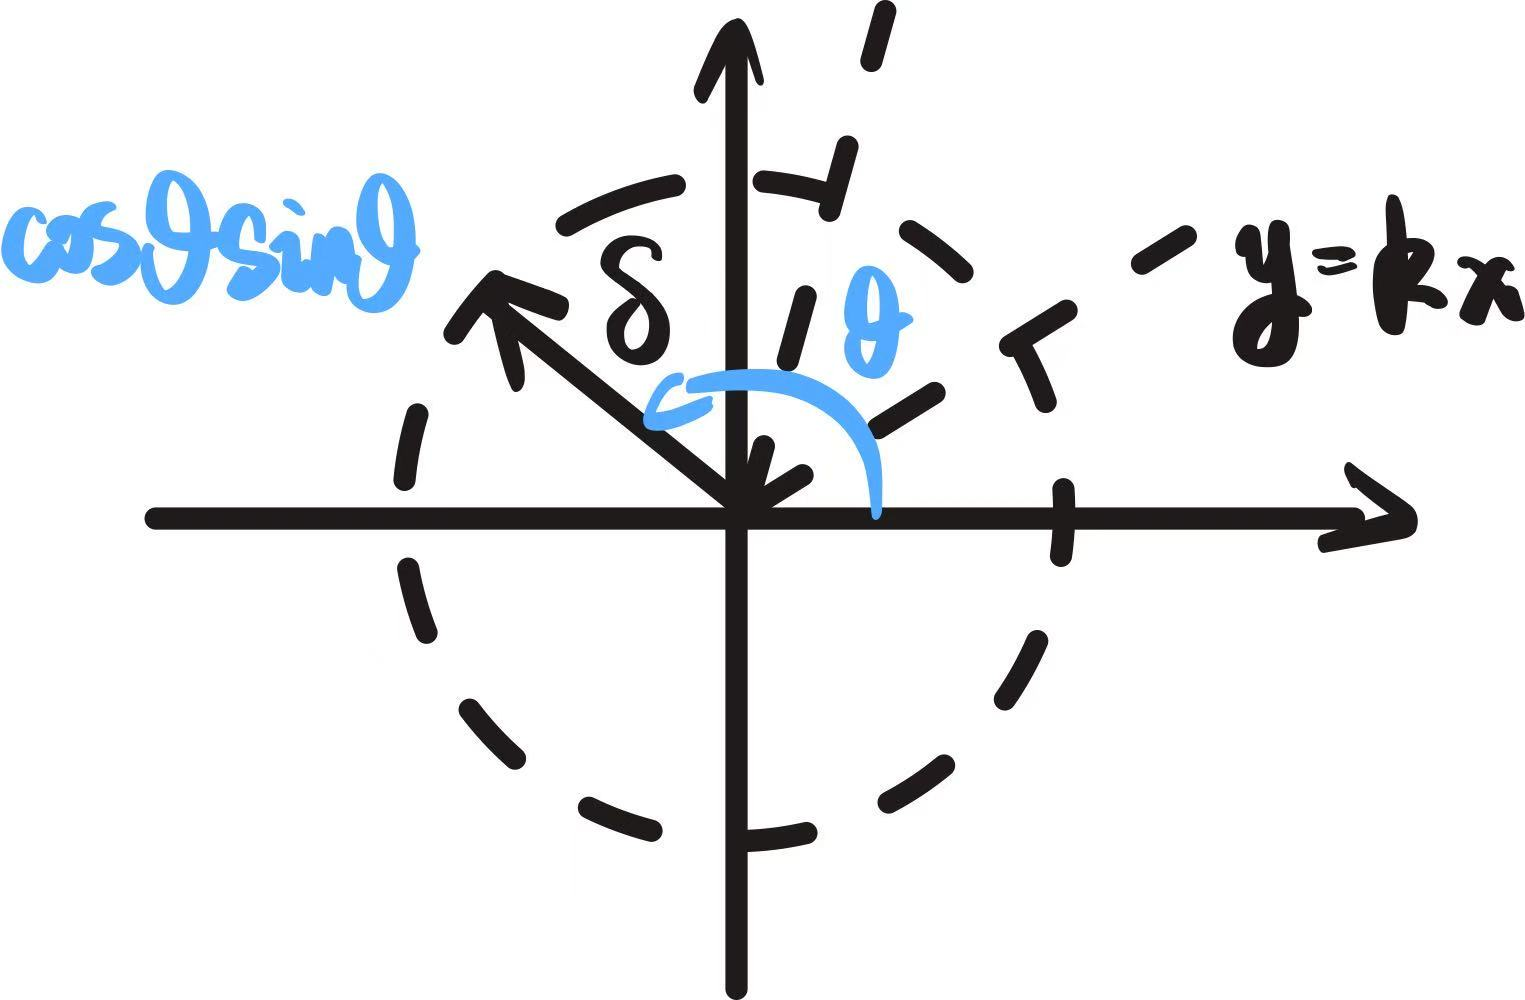
\includegraphics[height=2cm]{chapters/09/01/0301}}

    \begin{enumerate}
        \item Along the ray $y=kx$, $f(x,kx)=\frac{k}{1+k^2}\to\frac{k}{1+k^2}\,(x\to 0)$

              $\implies$ The limits are different along different rays

              $\implies\lim_{(x,y)\to(0,0)}f(x,y)$ does not exist
              \item\begin{align*}
                  \begin{cases}
                      x=r\cos\theta \\
                      y=r\sin\theta
                  \end{cases} & \implies f(\delta\cos\theta,\delta\sin\theta)=\cos\theta\sin\theta                                    \\
                                   & \implies\lim_{\delta\to 0}\sup_{M,M'\in\partial B(0,\delta)}\left|f(M)-f\left(M'\right)\right|=1 \\
                                   & \implies\lim_{(x,y)\to 0}f(x,y)\text{ does not exist}
              \end{align*}
    \end{enumerate}
\end{example}